% Created:      	05 Jun 2012
% Last modified: 	15 Aug 2012
%++++++++++++++++++++++++++++++++++++++++++++++++++++++++++++++++++++++++++++++++++++++++++++++++++++++++++++++++++++
\chapter{Sample chapter content}
\label{chapter1}
  \singlespace
  \minitoc
  \onehalfspace
  \acresetall

\section{Equations}
\label{sec:chap1:equations}

Equation with under-braces.
  \begin{equation}
  \label{eq:chap1:Leudeking_Piret_extended}
    r_{SMP} = \frac{d\,S_{SMP}}{dt} = \underbrace{\alpha \, \frac{d\,X}{dt}}_{\dfrac{d\,S_{UAP}}{dt}} + \underbrace{\beta \, X}_{\dfrac{d\,S_{BAP}}{dt}} + \underbrace{k_{hyd} \, X_{EPS}}_{\dfrac{d\,S_{BAP}}{dt}} - \underbrace{\sum_i \varepsilon_i \, p_i}_{\textrm{sinks}} + \underbrace{ \gamma\;f\left( c \, , \, \dfrac{dc}{dt} \right)}_{\dfrac{d\,S_{EAP}}{dt}}
  \end{equation} 
The \verb|aligned| environment
  \begin{equation}
  \label{eq:chap1:aligned}
  \begin{aligned}   
   \frac{\partial C}{\partial t} = \beta_L \, v_w \, \frac{\partial^2 C}{\partial x^2} - \alpha_R \, v_w \, \frac{\partial C}{\partial x} + k_s\,C^{N_s} - k_r\,S \\
   \frac{\partial d_p}{\partial t} = \frac{\partial S}{\partial t} \frac{d_p}{2\,\rho_s} \\
   \mathbf{S}(t=0) = 0 \\
   \mathbf{C}(t=0) = 0 \\
   \mathbf{d}_p(t=0) = d_{p0} \\
   C(x=0)=f\,\cfrac{v_s}{v_w}\,C_b \\
   \left. {\cfrac{\partial C}{\partial x}}\right|_{x=L} = 0
  \end{aligned}
  \end{equation}
Equation with the \verb|array| environment
  \begin{equation}
   f_T\left(x\,|\,\mu,\sigma,d_{p,cutoff}\right)=\left\{ 
   \begin{array}{r c l}
    K\, f\left(x\,|\,\mu,\sigma\right) & \mbox{for} & x<d_{p,cutoff} \\
    0 & \mbox{for} & x\ge d_{p,cutoff}
   \end{array} \right.
   \label{eq:chap1:pdf_truncated}
  \end{equation}
Example of long equation using the \verb|eqnarray| environment.
\begin{eqnarray}\nonumber
\displaystyle \frac{Q}{Q_0}&=&\frac{1}{\left(1+\tilde{\beta} Q_0 C_b t \right)^2} \; \exp \left( - \frac{\alpha C_b J_0 t}{1+\tilde{\beta} Q_0 C_b t} \right) \\
& + &\bigints\limits_0^t {\displaystyle\frac{\displaystyle\frac{\alpha C_b J_0}{\left( 1+\tilde{\beta} Q_0 C_b t_p \right)^2} \; \exp\left( -\displaystyle\frac{\alpha C_b J_0 t_p}{1+\tilde{\beta} Q_0 C_b t_p} \right)}{\sqrt{\left( \displaystyle\frac{R_{p0}}{R_m} + \left( 1+ \tilde{\beta} Q_0 C_b t_p \right)^2 \right)^2 + 2 \, \displaystyle\frac{f'R'\Delta P C_b}{\mu {R_m}^2} \left( t-t_p \right)}}} \; \mathrm{d}t
\label{eq:chap6:orsello_integral}
\end{eqnarray}

\section{Citations and footnotes}
\label{sec:chap1:citations}

\subsubsection{Single citations}

\verb|\citet{Metcalf2003}| produces \citet{Metcalf2003} \\
\verb|\citet[chapter 2]{Metcalf2003}| produces \citet[chapter 2]{Metcalf2003} \\
\verb|\citet[pp. 10-12]{Metcalf2003}| produces \citet[pp. 10-12]{Metcalf2003} \\
\verb|\citet[see][chap. 2]{Metcalf2003}| produces \citet[see][chap. 2]{Metcalf2003} \\

\noindent \verb|\citep{Olsson1999}| produces \citep{Olsson1999} \\
\verb|\citep[chapter 2]{Olsson1999}| produces \citep[chapter 2]{Olsson1999} \\
\verb|\citep[pp. 10-12]{Olsson1999}| produces \citep[pp. 10-12]{Olsson1999} \\
\verb|\citep[see][chap. 2]{Olsson1999}| produces \citep[see][chap. 2]{Olsson1999} \\

\subsubsection{Multiple citations}

\noindent \verb|\citet{Kaelin2009,Frolund1996,Eikelboom1983,Afonso2002}| produces \citet{Kaelin2009,Frolund1996,Eikelboom1983,Afonso2002} \\
\verb|\citep{Kaelin2009,Frolund1996,Eikelboom1983,Afonso2002}| produces \citep{Kaelin2009,Frolund1996,Eikelboom1983,Afonso2002} \\

More information about citation styles can be found in \url{http://en.wikibooks.org/wiki/LaTeX/Bibliography_Management}

Footnote inside the table using the \verb|savenotes| environment is shown in Table~\ref{tab:chap1:flux_stepping_identification_table}. Columns of Table~\ref{tab:chap1:flux_stepping_identification_table} have been automatically resized to occupy an entire width of the text.

  \begin{savenotes}
  \begin{table}[!h]
  \begin{footnotesize}
  \begin{center}
  \tabcolsep=0.15cm
  \setlength{\extrarowheight}{0pt}
  \renewcommand{\arraystretch}{1.3}
   \begin{tabular*}{\hsize}{@{\extracolsep{\fill}}l c c@{}}
   \toprule
      Identified lumped and single parameters & Unit & Value \\
      \midrule
      $\mu \, k_i \, S_{SMP}$ & mbar s$^{-1}$ (Lmh)$^{-2}$ & $2.306 \times 10^{-7}$ \\
      $b$ & (Lmh)$^{-1}$ & $7.991 \times 10^{-2}$ \\
      $\mu \, \alpha_c \, f_r \, X_{TSS}$ & mbar s$^{-1}$ (Lmh)$^{-2}$ & $7.391 \times 10^{-5}$ \\
      $\mu \, \alpha_c \, \dot{m}_{r,back}$ & mbar s$^{-1}$ (Lmh)$^{-1}$ & $1.884 \times 10^{-3}$ \\
      \midrule
      Recalculated single parameters & Unit & Value \\
      \midrule
      $k_i$ & m kg$^{-1}$ & $2.397 \times 10^{12}$ \\
      $\alpha_c$ \footnote{Calculated under assumption that $f_r=1$} & m kg$^{-1}$ & $5.061 \times 10^{15}$ \\
      $\dot{m}_{r,back}$ & kg m$^{-2}$ d$^{-1}$ & $1.040 \times 10^{-2}$ \\
   \bottomrule
   \end{tabular*} 
  \end{center}
  \end{footnotesize}
  \vspace{-0.5cm}
  \caption[List of parameters identified from the flux-stepping experiment.]{List of parameters identified from the $\frac{d \; \textrm{TMP}}{d \; t}$ vs. $J$ data generated from the flux-stepping experiment.}
  \label{tab:chap1:flux_stepping_identification_table}
\end{table} 
\end{savenotes}

Footnotes are created using the \verb|\footnote| command.\footnote{First footnote in the text.}. We can have multiple footnotes on a single page, however footnotes should best be avoided.\footnote{Second footnote in the text}.

\section{Lists}
\label{sec:chap1:lists}
\subsection{Enumerate lists}
\label{subsec:chap1:enumerate}

\subsubsection{Arabic enumerators (default)}
\begin{enumerate}
\item First item.
\item Second item. 
\item Third item.
\end{enumerate}

\subsubsection{Roman enumerators}
\begin{enumerate}[I]
\item First item.
\item Second item. 
\item Third item.
\end{enumerate}

\subsubsection{Small alpha-characters within brackets}
\begin{enumerate}[(a)]
\item First item.
\item Second item. 
\item Third item.
\end{enumerate}

\subsection{Itemize lists}
\label{subsec:chap1:itemize}

% Four levels in the itemizate environment may be changed to suit specific needs
\renewcommand{\labelitemi}{$\bullet$}
\renewcommand{\labelitemii}{$\diamond$}
\renewcommand{\labelitemiii}{$\ast$}
\renewcommand{\labelitemiv}{$\cdot$}

\begin{itemize}
 \item First item.
 \item Second item.
 \item Third item.
\end{itemize}

\subsection{Description lists}
\label{subsec:chap1:description}

\begin{description}
 \item[Physics] Physics is awesome.
 \item[Geology] Geology is not science.
 \item[Social Science] Social ``Science''.
\end{description}

\subsection{Nested lists}
\label{subsec:chap1:nested_lists}

\begin{itemize}
\item First level, itemize first item.
  \begin{itemize}
   \item Second level, itemize, first item.
   \item Second level, itemize, second item.
    \begin{enumerate}
     \item Third level, enumerate, first item.
     \item Third level, enumerate, second item.
    \end{enumerate}
    \begin{itemize}
    \item Third level, itemize, first item.
    \item Third level, itemize, second item.
    \end{itemize}
  \item Second level, itemize, third item.
  \end{itemize}
\item First level, itemize, third item.
\end{itemize}

\section{Computer code and flow diagrams}
\label{sec:chap1:computer_code}

Presentation of C-code using the \verb|listings| package and the \verb|lstlisting| environment.

\lstset{escapechar=@,style=customc}
\begin{lstlisting}
#include <stdio.h>
 
int main()
{
   int array[100], search, c, n, count = 0;
 
   printf("Enter the number of elements in array\n");
   scanf("%d",&n);
 
   printf("Enter %d numbers\n", n);
 
   for ( c = 0 ; c < n ; c++ )
      scanf("%d",&array[c]);
 
   printf("Enter the number to search\n");
   scanf("%d",&search);
 
   for ( c = 0 ; c < n ; c++ )
   {
      if ( array[c] == search )    
      {
         printf("%d is present at location %d.\n", search, c+1);
	 count++;
      }
   }
   if ( count == 0 )
      printf("%d is not present in array.\n", search);
   else
      printf("%d is present %d times in array.\n", search, count);
 
   return 0;
}
\end{lstlisting}

For more information about the \verb|listings| package, please visit \url{http://en.wikibooks.org/wiki/LaTeX/Source_Code_Listings}.

Algorithm ``pseudocode'' can be displayed using the \verb|algorithm| and \verb|algorithmic| environments as demonstrate in Algorithm~\ref{alg:chap1:alg1}.
\begin{algorithm}                      % enter the algorithm environment
\caption{Calculate $y = x^n$.}          % give the algorithm a caption
\label{alg:chap1:alg1}                 % and a label for \ref{} commands later in the document
\begin{algorithmic}                    % enter the algorithmic environment
    \REQUIRE $n \geq 0 \vee x \neq 0$
    \ENSURE $y = x^n$
    \STATE $y \Leftarrow 1$
    \IF{$n < 0$}
        \STATE $X \Leftarrow 1 / x$
        \STATE $N \Leftarrow -n$
    \ELSE
        \STATE $X \Leftarrow x$
        \STATE $N \Leftarrow n$
    \ENDIF
    \WHILE{$N \neq 0$}
        \IF{$N$ is even}
            \STATE $X \Leftarrow X \times X$
            \STATE $N \Leftarrow N / 2$
        \ELSE[$N$ is odd]
            \STATE $y \Leftarrow y \times X$
            \STATE $N \Leftarrow N - 1$
        \ENDIF
    \ENDWHILE
\end{algorithmic}
\end{algorithm}

A lot of artwork including block diagrams as well as more complex vector graphics can be created using the \verb|tickz| package. Examples of such diagrams are shown in Figure~\ref{fig:chap1:tikzpicture1} on page~\pageref{fig:chap1:tikzpicture1} and Figure~\ref{fig:chap1:tikzpicture2} on page~\pageref{fig:chap1:tikzpicture2}. For more information, the reader is referred to \url{http://www.texample.net/tikz/examples/all/?page=1}.

% Define block styles
\tikzstyle{decision} = [diamond, draw, fill=blue!20, 
    text width=4.5em, text badly centered, node distance=3cm, inner sep=0pt]
\tikzstyle{block} = [rectangle, draw, fill=blue!20, 
    text width=5em, text centered, rounded corners, minimum height=4em]
\tikzstyle{line} = [draw, -latex']
\tikzstyle{cloud} = [draw, ellipse,fill=red!20, node distance=3cm,
    minimum height=2em]

\begin{figure}
\centering
\begin{tikzpicture}[node distance = 2cm, auto]
    % Place nodes
    \node [block] (init) {initialize model};
    \node [cloud, left of=init] (expert) {expert};
    \node [cloud, right of=init] (system) {system};
    \node [block, below of=init] (identify) {identify candidate models};
    \node [block, below of=identify] (evaluate) {evaluate candidate models};
    \node [block, left of=evaluate, node distance=3cm] (update) {update model};
    \node [decision, below of=evaluate] (decide) {is best candidate better?};
    \node [block, below of=decide, node distance=3cm] (stop) {stop};
    % Draw edges
    \path [line] (init) -- (identify);
    \path [line] (identify) -- (evaluate);
    \path [line] (evaluate) -- (decide);
    \path [line] (decide) -| node [near start] {yes} (update);
    \path [line] (update) |- (identify);
    \path [line] (decide) -- node {no}(stop);
    \path [line,dashed] (expert) -- (init);
    \path [line,dashed] (system) -- (init);
    \path [line,dashed] (system) |- (evaluate);
\end{tikzpicture}
\caption{Flow diagram created with the `tickz' package.}
\label{fig:chap1:tikzpicture1}
\end{figure}

\begin{figure}
\centering
% A simple graph with straight and bend arrows and loops
% Stefan Kottwitz
\begin{tikzpicture}[->,>=stealth',shorten >=1pt,auto,node distance=3cm,
  thick,main node/.style={circle,fill=blue!20,draw,font=\sffamily\Large\bfseries}]

  \node[main node] (1) {1};
  \node[main node] (2) [below left of=1] {2};
  \node[main node] (3) [below right of=2] {3};
  \node[main node] (4) [below right of=1] {4};

  \path[every node/.style={font=\sffamily\small}]
    (1) edge node [left] {0.6} (4)
        edge [bend right] node[left] {0.3} (2)
        edge [loop above] node {0.1} (1)
    (2) edge node [right] {0.4} (1)
        edge node {0.3} (4)
        edge [loop left] node {0.4} (2)
        edge [bend right] node[left] {0.1} (3)
    (3) edge node [right] {0.8} (2)
        edge [bend right] node[right] {0.2} (4)
    (4) edge node [left] {0.2} (3)
        edge [loop right] node {0.6} (4)
        edge [bend right] node[right] {0.2} (1);
\end{tikzpicture}
\caption{Simple graph created with the `tickz' package.}
\label{fig:chap1:tikzpicture2}
\end{figure}

\section{Artwork}
\label{sec:chap1:artwork}

The document is designed to be compiled using the \emph{latex$\rightarrow$ bibtex$\rightarrow$ latex$\rightarrow$ latex $\rightarrow$ dvips$\rightarrow$ pspdf} compilation sequence. Hence, the external graphic files for inclusion need to be prepared in the .EPS format.

\subsection{Tables}
\label{subsec:chap1:tables}

Example of a large table occupying an entire size A4 page is shown in Table~\ref{tab:chap1:petersen_matrix_cesasm3} which uses the \verb|sidewaystable| environment.

    \begin{sidewaystable}[htbp]
    \caption[Stoichiometric (Petersen) and composition matrix.]{Stoichiometric (Petersen) and composition matrix, \emph{j}: process, \emph{i}: component.}
    \vspace{-0.5cm}
    \begin{tiny}
    \begin{center}
    \tabcolsep=0.12cm
    \extrarowheight = 5.5pt
    \begin{tabular}{ l p{4cm} c c c c c c c c c c c c c c c c}
    \toprule
    & Model components \emph{i} & 1 & 2 & 3 & 4 & 5 & 6 & 7 & 8 & 9 & 10 & 11 & 12 & 13 & 14 & 15 & 16 \\ \midrule
    $\emph{j}$ & Processes & $S_O$ & $S_I$ & $S_S$ & $S_{NH}$ & $S_{N2}$ & $S_{NO}$ & $S_{HCO}$ & $S_{BAP}$ & $S_{UAP}$ & $X_I$ & $X_S$ & $X_H$ & $X_{STO}$ & $X_A$ & $X_{EPS}$ & $X_{TSS}$ \\
    & \multicolumn{17}{l}{\emph{Heterotrophic organisms}} \\
    $p_1$ & Hydrolysis & & $f_{S_I}$ & $1-f_{S_I}$ & $y_1$ & & & $z_{1}$ & & & & -1 & & & & & $t_{1}$ \\
    $p_{2,a}$ & Aerobic storage of $S_S$ & $x_{2a}$ & & -1 & $y_{2a}$ & & & $z_{2a}$ & & & & & & \begin{tabular}{c}$Y_{STO,O_2}-$\\$f_{EPS,STO}$ \end{tabular} & & $f_{EPS,STO}$ & $t_{2a}$ \\
    $p_{2,b}$ & Aerobic storage of $S_{BAP}$ & $x_{2b}$ & & & $y_{2b}$ & & & $z_{2b}$ & -1 & & & & & \begin{tabular}{c}$Y_{STO,SMP,O_2}-$\\$f_{EPS,STO}$ \end{tabular} & & $f_{EPS,STO}$ & $t_{2b}$ \\
    $p_{2,c}$ & Aerobic storage of $S_{UAP}$ & $x_{2c}$ & & & $y_{2c}$ & & & $z_{2c}$ & & -1 & & & \begin{tabular}{c}$Y_{STO,SMP,O_2}-$\\$f_{EPS,STO}$ \end{tabular} & & & $f_{EPS,STO}$ & $t_{2c}$ \\
    $p_{3,a}$ & Anoxic storage of $S_S$ & & & -1 & $y_{3a}$ & $-x_{3a}$ & $x_{3a}$ & $z_{3a}$ & & & & & & \begin{tabular}{c}$Y_{STO,NO}-$\\$f_{EPS,STO}$ \end{tabular} & & $f_{EPS,STO}$ & $t_{3a}$ \\
    $p_{3,b}$ & Anoxic storage of $S_{BAP}$ & & & & $y_{3b}$ & $-x_{3b}$ & $x_{3b}$ & $z_{3b}$ & -1 & & & & &  \begin{tabular}{c}$Y_{STO,SMP,NO}-$\\$f_{EPS,STO}$ \end{tabular} & & $f_{EPS,STO}$ & $t_{3b}$ \\
    $p_{3,b}$ & Anoxic storage of $S_{UAP}$ & & & & $y_{3c}$ & $-x_{3c}$ & $x_{3c}$ & $z_{3c}$ & & -1 & & &  \begin{tabular}{c}$Y_{STO,SMP,NO}-$\\$f_{EPS,STO}$\end{tabular} & & & $f_{EPS,STO}$ & $t_{3c}$ \\
    $p_4$ & Aerobic growth & $x_{4}$ & & & $y_4$ & & & $z_{4}$ & & $\gamma_H/Y_{H,O_2}$ & & & $1-f_{EPS,h}$ & $-1/Y_{H,O_2}$ & & $f_{EPS,h}$ & $t_{4}$ \\
    $p_5$ & Anoxic growth & & & & $y_5$ & $-x_{5}$ & $x_{5}$ & $z_{5}$ & & $\gamma_H/Y_{H,NO}$ & & & $1-f_{EPS,h}$ & $-1/Y_{H,NO}$ & & $f_{EPS,h}$ & $t_{5}$ \\
    $p_6$ & Aerobic endogenous respiration & $x_{6}$ & & & $y_6$ & & & $z_{6}$ & $f_{BAP}$ & & $f_{X_I}$ & & -1 & & & $f_{EPS,dh}$ & $t_{6}$ \\
    $p_7$ & Anoxic endogenous respiration & & & & $y_7$ & $-x_{7}$ & $x_{7}$ & $z_{7}$ & $f_{BAP}$ & & $f_{X_I}$ & & -1 & & & $f_{EPS,dh}$ & $t_{7}$ \\
    $p_8$ & Aerobic respiration of $X_{STO}$ & $x_{8}$ & & & & & & & & & & & & -1 & & & $t_{8}$	\\
    $p_9$ & Anoxic respiration of $X_{STO}$ & & & & & $-x_{9}$ & $x_{9}$ & $z_{9}$ & & & & & & -1 & & & $t_{9}$ \\
    & \multicolumn{17}{l}{\emph{Autotrophic organisms}} \\
    $p_{10}$ & Nitrification & $x_{10}$ & & & $y_{10}$ & & $1/Y_A$ & $z_{10}$ & & $\gamma_A/Y_A$ & & & & & $1-f_{EPS,a}$ & $f_{EPS,a}$ & $t_{10}$ \\
    $p_{11}$ & Aerobic endogenous respiration & $x_{11}$ & & & $y_{11}$ & & & $z_{11}$ & $f_{BAP}$ & & $f_{X_I}$ & & & & -1 & $f_{EPS,da}$ & $t_{11}$ \\
    $p_{12}$ & Anoxic endogenous respiration & & & & $y_{12}$ & $-x_{12}$ & $x_{12}$ & $z_{12}$ & $f_{BAP}$ & & $f_{X_I}$ & & & & -1 & $f_{EPS,da}$ & 	$t_{12}$ \\
    & \multicolumn{17}{l}{\emph{\acs{EPS} and $X_I$ hydrolysis}} \\
    $p_{13}$ & Hydrolysis of $X_{EPS}$ & & & $f_S$ & & & & & $1-f_S$ & & & & & & & -1 & $t_{13}$ \\
    $p_{14}$ & Hydrolysis of $X_{I}$ & & $f_{I,I}$ & $1-f_{I,I}$ & $f_{N,I}$ & & & & & & $-1$ & & & & & & $t_{14}$ \\ \midrule
    1 & ThOD (g ThOD) & -1 & 1 & 1 & & $-24/14$ & $-64/14$ & & 1 & 1 & 1 & 1 & 1 & 1 & 1 & 1 & \\
    2 & Nitrogen (g N) & & $i_{N,S_{I}}$ & $i_{N,S_{S}}$ & 1 & 1 & 1 & & $i_{N,S_{BAP}}$ & & $i_{N,X_I}$ & $i_{N,X_S}$ & $i_{N,BM}$ & & $i_{N,BM}$ & $i_{N,X_{EPS}}$ & \\
    3 & Ionic charge (Mole$^+$) & & & & $1/14$ & & $-1/14$ & -1 & & 	& & & & & & & \\
    4 & TSS (g TSS) & & & & & & & & & & $i_{TSS,X_I}$ & $i_{TSS,X_S}$ & $i_{TSS,BM}$ & $i_{TSS,STO}$ & $i_{TSS,BM}$ & $i_{TSS,EPS}$ & 1 \\ \bottomrule
    \end{tabular}
    \end{center}
    This model assumes that ThOD is identical to the measured \ac{COD}. 1 g$S_O$ = -1 gThOD, 1 g$S_{NH}$ = 0 gThOD, 1g$S_{NO}$ = -64/14 gThOD, 1 g$S_{N_2}$ = -24/14 gThOD. \\
    \end{tiny}
    \label{tab:chap1:petersen_matrix_cesasm3}
    \end{sidewaystable}

An exemplary table which incorporates the \verb|\multirow| and \verb|\multicolumn| commands is shown in Table~\ref{tab:chap1:transport_membrane_simulation_parameters}.
    
  \begin{table}
  \begin{footnotesize}
  \begin{center}
  \tabcolsep=0.07cm
  \setlength{\extrarowheight}{0pt}
   \begin{tabular}{l c c c c}
   \toprule
   \multirow{2}[3]{*}{Parameter} & \multirow{2}[3]{*}{Description} & \multirow{2}[3]{*}{Unit} & \multicolumn{2}{c}{Value} \\
   \cmidrule(r){4-5}
   & & & Simu 1 & Simu 2 \\
   \midrule
    Membrane thickness & $L$ & $\mu$m &  \multicolumn{2}{c}{$100$} \\
    Fraction of \ac{SMP} in permeate & $f$ & -- &  \multicolumn{2}{c}{$1$} \\
    \ac{SMP} retardation coefficient & $\alpha_R$ & -- & \multicolumn{2}{c}{$0.5$} \\
    \ac{SMP} dispersion factor & $\beta_L$ & -- & $1$ & $\left[ 0.5,3,9 \right]$ \\
    Permeate flux & $J$ & L m$^{-2}$ h$^{-1}$ & $\left[ 20,40 \right]$ & $20$ \\
    Initial \ac{SMP} concentration in the membrane & $C_0$ & kg m$^{-3}$ & \multicolumn{2}{c}{$0$} \\
    Bulk \ac{SMP} concentration & $C_b$ & kg m$^{-3}$ & \multicolumn{2}{c}{$200$} \\ 
    Membrane porosity & $\varepsilon$ & -- & \multicolumn{2}{c}{$0.6$} \\
    Mean pore diameter & $d_p$ & $\mu$m & \multicolumn{2}{c}{$0.1$} \\
    Density of proteins & $\rho_p$ & kg m$^{-3}$ & \multicolumn{2}{c}{$1.35$} \\
    Sorption rate & $k_s$ & s$^{-1}$ &  \multicolumn{2}{c}{$2 \cdot 10^{-6}$} \\
    Desorption rate & $k_r$ & s$^{-1}$ & \multicolumn{2}{c}{$1 \cdot 10^{-6}$} \\
    Non-linearity coefficient in the sorption model & $N_s$ & -- & \multicolumn{2}{c}{$1$} \\
    \bottomrule
   \end{tabular} 
  \end{center}
  \end{footnotesize}
  \vspace{-0.5cm}
  \caption[Parameters used for simulation of SMP transport through a membrane.]{Parameters used for the simulation of \ac{SMP} transport through a membrane.}
  \label{tab:chap1:transport_membrane_simulation_parameters}
  \end{table} 
    
\subsection{Figures}
\label{subsec:chap1:figures}

Example of a large figure which uses an entire page is shown in Figure~\ref{fig:chap1:simplified_model_mbr}.

\begin{figure}[htbp]
\centering
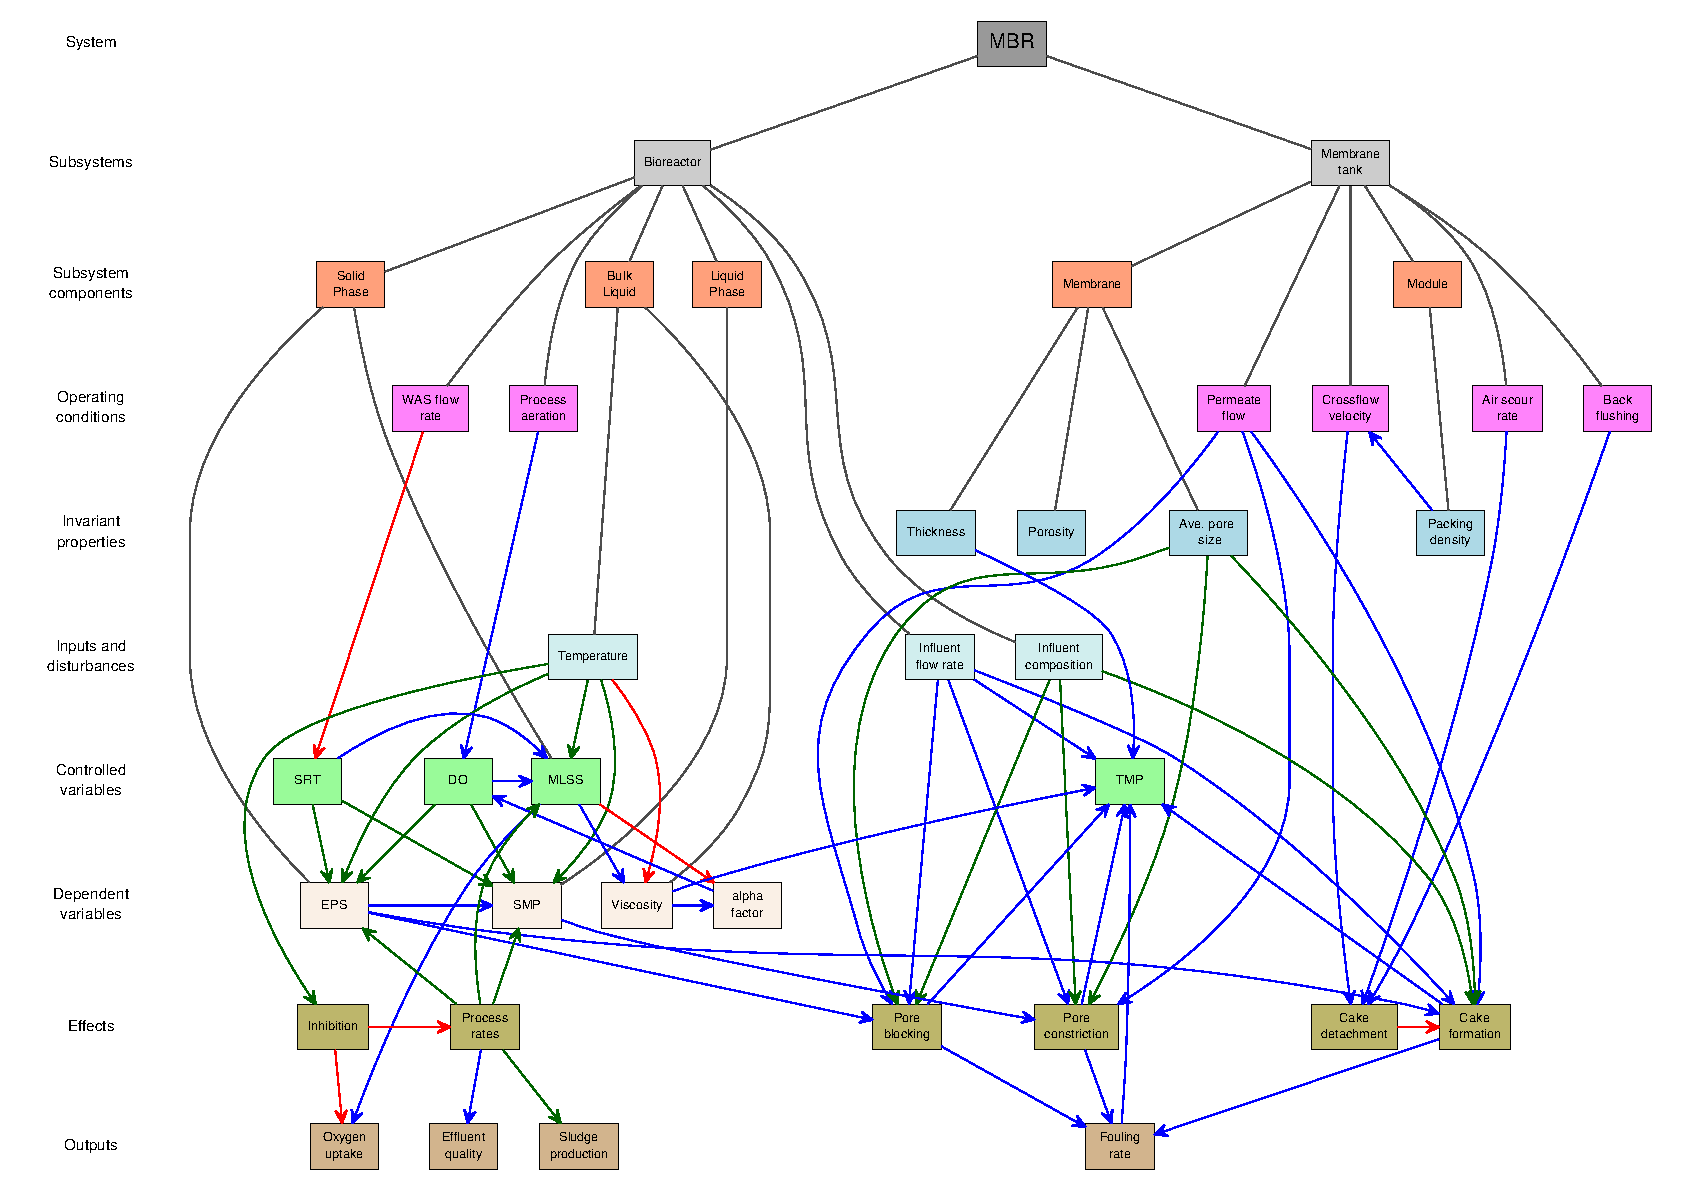
\includegraphics[width=1.4\textwidth,angle=90]{graphics/membranes_reduced.eps}
\caption[Graphical representation of a simplified MBR modelling problem.] {Graphical representation of a simplified \ac{MBR} modelling problem.}
\label{fig:chap1:simplified_model_mbr}
\end{figure} 

Two figures, next to each other obtained by nesting \verb|subfigure| inside the \verb|figure| environment.

  \begin{figure}
	  \centering
	  \begin{subfigure}[b]{0.48\textwidth}
		  \centering
		  \includegraphics[width=\textwidth]{graphics/dPdt_vs_flux_irrev_fouling.eps}
% 		  \caption{Rate of \ac{TMP} increase due to irreversible fouling at different permeate fluxes}
		  \caption{}
		  \label{fig:chap1:pressure_increase_irrev_fouling}
	  \end{subfigure}
	  %add desired spacing between images, e. g. ~, \quad, \qquad etc. 
	    %(or a blank line to force the subfigure onto a new line)
	  \begin{subfigure}[b]{0.48\textwidth}
		  \centering
		  \includegraphics[width=\textwidth]{graphics/dPdt_vs_flux_rev_fouling.eps}
% 		  \caption{Rate of \ac{TMP} increase due to reversible fouling at different permeate fluxes}
		  \caption{}
		  \label{fig:chap1:pressure_increase_rev_fouling}
	  \end{subfigure}%
	  %add desired spacing between images, e. g. ~, \quad, \qquad etc. 
	    %(or a blank line to force the subfigure onto a new line)
	  \caption[TMP increase in time due to irreversible and reversible fouling and flux.]{\acs{TMP} increase in time due to (a) irreversible and (b) reversible fouling and flux rate.}
	  \label{fig:chap1:TMP_increse_flux}
  \end{figure} 

  Schematic representation of the overall structure of the thesis is presented in Figure~\ref{fig:chap1:thesis_structure}
  
  \begin{figure}[htp]
  \centering
  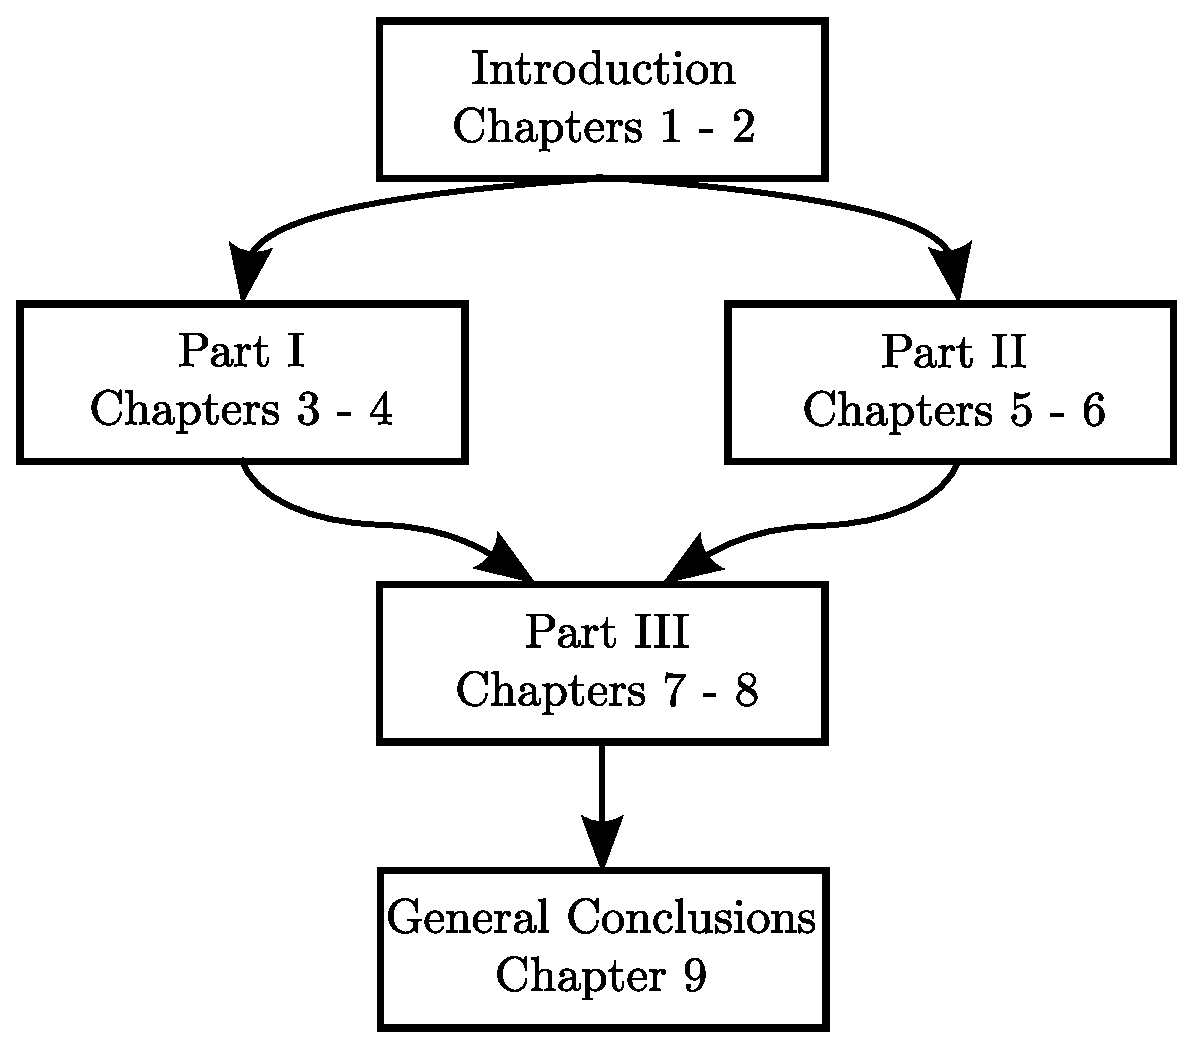
\includegraphics[width=0.6\textwidth]{graphics/thesis_structure_introduction.eps}
  \caption[Schematic representation of the overall structure of the thesis.] {Schematic representation of the overall structure of the thesis.}
  \label{fig:chap1:thesis_structure}
  \end{figure} 

\section{Theorems \& Definitions}
\label{sec:chap1:definitions}

\subsection{Example 1}
\label{sec:chap1:theorem_definition_example_1}

It is well known how to solve polynomial equations of the first
degree.  For a first degree equation $ax+b=0$ with $a\neq 0$ the
solution is $x=-b/a$.  We now look at solving $ax^2+bx+c=0$.

\begin{theorem}
The equation $ax^2+bx+c=0$ with $a\neq 0$ as the solutions
$$
x=\frac{-b\pm \sqrt{b^2-4ac}}{2a}
$$
\end{theorem}

\begin{proof}
We use the method of completing the square to rewrite $ax^2+bx+c$.
\begin{align*}
ax^2+bx+c&=a\left( x^2 + \frac{b}{a}x+\right)+c \\
  &=a\left( x^2 + \frac{b}{a}x+ \left(\frac{b}{2a}\right)^2
     -\left(\frac{b}{2a}\right)^2 +\right)+c \\
  &=a\left( x+\frac{b}{2a}\right)^2 -  a\left(\frac{b}{2a}\right)^2+c\\
  &= a\left( x+\frac{b}{2a}\right)^2- \frac{b^2-4ac}{4a}.
\end{align*}
Therefore $ax^2+bx+c=0$ can be rewritten as 
$$
a\left( x+\frac{b}{2a}\right)^2- \frac{b^2-4ac}{4a}=0,
$$
which can in turn  be rearranged as
$$
\left( x+\frac{b}{2a}\right)^2= \frac{b^2-4ac}{4a^2}.
$$
Taking square roots gives
$$
x+\frac{b}{2a}= \frac{\pm \sqrt{b^2-4ac}}{2a}
$$
which implies
$$
x=\frac{-b\pm \sqrt{b^2-4ac}}{2a}
$$
as required.
\end{proof}

\subsection{Example 2}
\label{sec:chap1:theorem_definition_example_2}

\renewcommand{\qed}{\nobreak \ifvmode \relax \else
      \ifdim\lastskip<1.5em \hskip-\lastskip
      \hskip1.5em plus0em minus0.5em \fi \nobreak
      \vrule height0.75em width0.5em depth0.25em\fi}

\begin{definition}
Let $H$ be a subgroup of a group~$G$.  A \emph{left coset} of $H$ in $G$ is a subset of $G$ that is of the form $xH$, where $x \in G$ and $xH = \{ xh : h \in H \}$. Similarly a \emph{right coset} of $H$ in $G$ is a subset of $G$ that is of the form $Hx$, where $Hx = \{ hx : h \in H \}$
\end{definition}

Note that a subgroup~$H$ of a group $G$ is itself a left coset of $H$ in $G$.

\begin{lemma}
\label{LeftCosetsDisjoint}
Let $H$ be a subgroup of a group $G$, and let $x$ and $y$ be elements of $G$.  Suppose that $xH \cap yH$ is non-empty. Then $xH = yH$.
\end{lemma}

\begin{proof}
Let $z$ be some element of $xH \cap yH$.  Then $z = xa$ for some $a \in H$, and $z = yb$ for some $b \in H$. If $h$ is any element of $H$ then $ah \in H$ and $a^{-1}h \in H$, since $H$ is a subgroup of $G$. But $zh = x(ah)$ and $xh = z(a^{-1}h)$ for all $h \in H$. Therefore $zH \subset xH$ and $xH \subset zH$, and thus $xH = zH$.  Similarly $yH = zH$, and thus $xH = yH$, as required.\qed
\end{proof}

\begin{lemma}
\label{SizeOfLeftCoset}
Let $H$ be a finite subgroup of a group $G$.  Then each left coset of $H$ in $G$ has the same number of elements as $H$.
\end{lemma}

\begin{proof}
\label{chap1:proof:proof1}
Let $H = \{ h_1, h_2,\ldots, h_m\}$, where $h_1, h_2,\ldots, h_m$ are distinct, and let $x$ be an element of $G$.  Then the left coset $xH$ consists of the elements $x h_j$ for $j = 1,2,\ldots,m$. Suppose that $j$ and $k$ are integers between
$1$ and $m$ for which $x h_j = x h_k$. 
Then $h_j = x^{-1} (x h_j) = x^{-1} (x h_k) = h_k$, and thus $j = k$, since $h_1, h_2,\ldots, h_m$ are distinct.  It follows that the elements $x h_1, x h_2,\ldots, x h_m$ are distinct.
We conclude that the subgroup~$H$ and the left coset $xH$ both have $m$ elements, as required.\qed
\end{proof}

\begin{theorem}
\emph{(Lagrange's Theorem)}
\label{Lagrange}
Let $G$ be a finite group, and let $H$ be a subgroup of $G$.  Then the order of $H$ divides the order of $G$.
\end{theorem}

\begin{proof}
\label{chap1:proof:proof2}
Each element~$x$ of $G$ belongs to at least one left coset of $H$ in $G$ (namely the coset $xH$), and no element can belong to two distinct left cosets of $H$ in $G$ (see Lemma~\ref{LeftCosetsDisjoint}).  Therefore every element of $G$ belongs to exactly one left coset of $H$. 
Moreover each left coset of $H$ contains $|H|$ elements (Lemma~\ref{SizeOfLeftCoset}).  Therefore $|G| = n |H|$, where $n$ is the number of left cosets of $H$ in $G$. The result follows.\qed
\end{proof}

\section{New commands}
\label{sec:chap1:new_commands}

We can define new \LaTeX commands to speed-up the writing process. Such new commands have been defined in \verb|style.tex| and are listed below. 
\lstset{escapechar=@,style=customlatex}
\begin{lstlisting}
\newcommand{\sq}{\ensuremath{^2~}}
\newcommand{\sqs}{\ensuremath{^2}}
\newcommand{\cb}{\ensuremath{^3~}}
\newcommand{\cbs}{\ensuremath{^3}}
\newcommand{\x}{\ensuremath{\times}}
\newcommand{\degr}{\ensuremath{^\circ}~}
\newcommand{\degrs}{\ensuremath{^\circ}}
\newcommand{\prox}{$\approx$}
\newcommand{\degc}{$^{\circ}$C~}
\newcommand{\degcs}{$^{\circ}$C}
\end{lstlisting}

We can use these new commands and avoid writing long expressions in the text, i.e. 2\sq instead of 2$^2$, 20\degc instead of 20$^\textrm{o}$C, \prox50~mm instead of $\approx$50~mm.

\section{Referencing and acronyms}
\label{sec:chap1:referencing}

Almost any object in \LaTeX~can be referred to by its label description defined in the \verb|\label| command. Since, in large documents, it is possible to create duplicate labels referring to different types of objects, e.g. the same label may be accidentally given to a figure and a table, it is common practice among \LaTeX~users to add a few letters to the label to describe what you are referencing, i.e. \textbf{chap:} for a chapter, \textbf{sec:} for a section, \textbf{fig:} for a figure, \textbf{tab:} for a table, \textbf{eq:} for an equation, \textbf{lst:} for code listing, \textbf{itm:} for an enumerated list. item. Example references are listed as follows: Lemma~\ref{LeftCosetsDisjoint} on page~\pageref{LeftCosetsDisjoint} and Lemma~\ref{SizeOfLeftCoset} on page~\pageref{SizeOfLeftCoset}. Figure~\ref{fig:chap1:thesis_structure} on page~\pageref{fig:chap1:thesis_structure}. Table~\ref{tab:chap1:transport_membrane_simulation_parameters} on page \pageref{tab:chap1:transport_membrane_simulation_parameters}. Section~\ref{sec:chap1:new_commands}.

The \verb|acronym| package helps you manage acronyms and acronym lists in your documents. You can define each acronym within a special acronym environment and then use macros in the text to define how each occurrence of the acronym will appear when you typeset the document.

\noindent First occurrence of \verb|\ac{NH4-N}| will expand and identify the acronym the first time. Hence, it will produce:~\ac{NH4-N}. 

\noindent Second and further occurrences of \verb|\ac{NH4-N}| will produce:~\ac{NH4-N}.

\noindent \verb|\acf{NH4-N}| uses the full name of the acronym, i.e.~\acf{NH4-N}.

\noindent \verb|\acs{NO3-N}| uses the short version of the acronym, i.e.~\acs{NO3-N}.

\noindent \verb|\acl{PnID}| expands the acronym without using the acronym itself, i.e. \acs{PnID}.

\noindent \verb|\acp{PnID}| lists an acronym in plural, i.e. \acp{PnID}.

\noindent \verb|\acfp{PnID}| lists an acronym in a plural full form, i.e. \acfp{PnID}.

\noindent \verb|\acsp{PnID}| lists an acronym in a plural short form, i.e. \acsp{PnID}.